\section{Objective}
\label{sec:Objective}
The goal of the experiment is to familiarize oneself with the workings of interferometry and a sagnac 
inferometer. Using this knowledge and inferometer the refractorary index of glass and air is determinated. 
\section{Theoratical Background}
\label{sec:Theorie}
\subsection{Coherance, polarisation  and interference of light}
The coherance of a wave describes how well the phase is mantained throughout the propagation. The temporal coherance measures how long a 
wave holds the same shape periodically and the spatial coherance measures the phase unity across different points in the wavefront.
The coherance is linked to the spectral bandwidth the lightsource has. In general a narrow bandwidth leads to a long coherance time.
The degree of coherance a wave can have is ranging from 0 (fully incoherant) to 1 (fully coherant). 
Another property of light is its polarisation. Light can be linear polarized, circular or eliptically polarized or unpolarized. 
In case of a linear polarized light the electric field osciallates in a fixed plane. If it is circular or eliptically polarized the 
electric field rotates over time around the direction of propagation. 
For two beams to interfere with each other they both must be coherant, overlapping spatially and have the same polarisation direction or
compounts in the same direction. Therefor beams with polarisation that is perpendicular to each other cannot interfere. 

\subsection{Sagnac-Interferometer}
The Sagnac-Interferometer is a type of interferometer where the initial light beam is split into two by using an polarizing beam-splitter 
cube. The two beams propagate along the same paths just in opposite directions and are recombined afterwards. 
The topology of the Sagnac-Interferometer can be seen in \autoref{pic:Sagnac-Interferometer}.

\begin{figure}
    \centering
    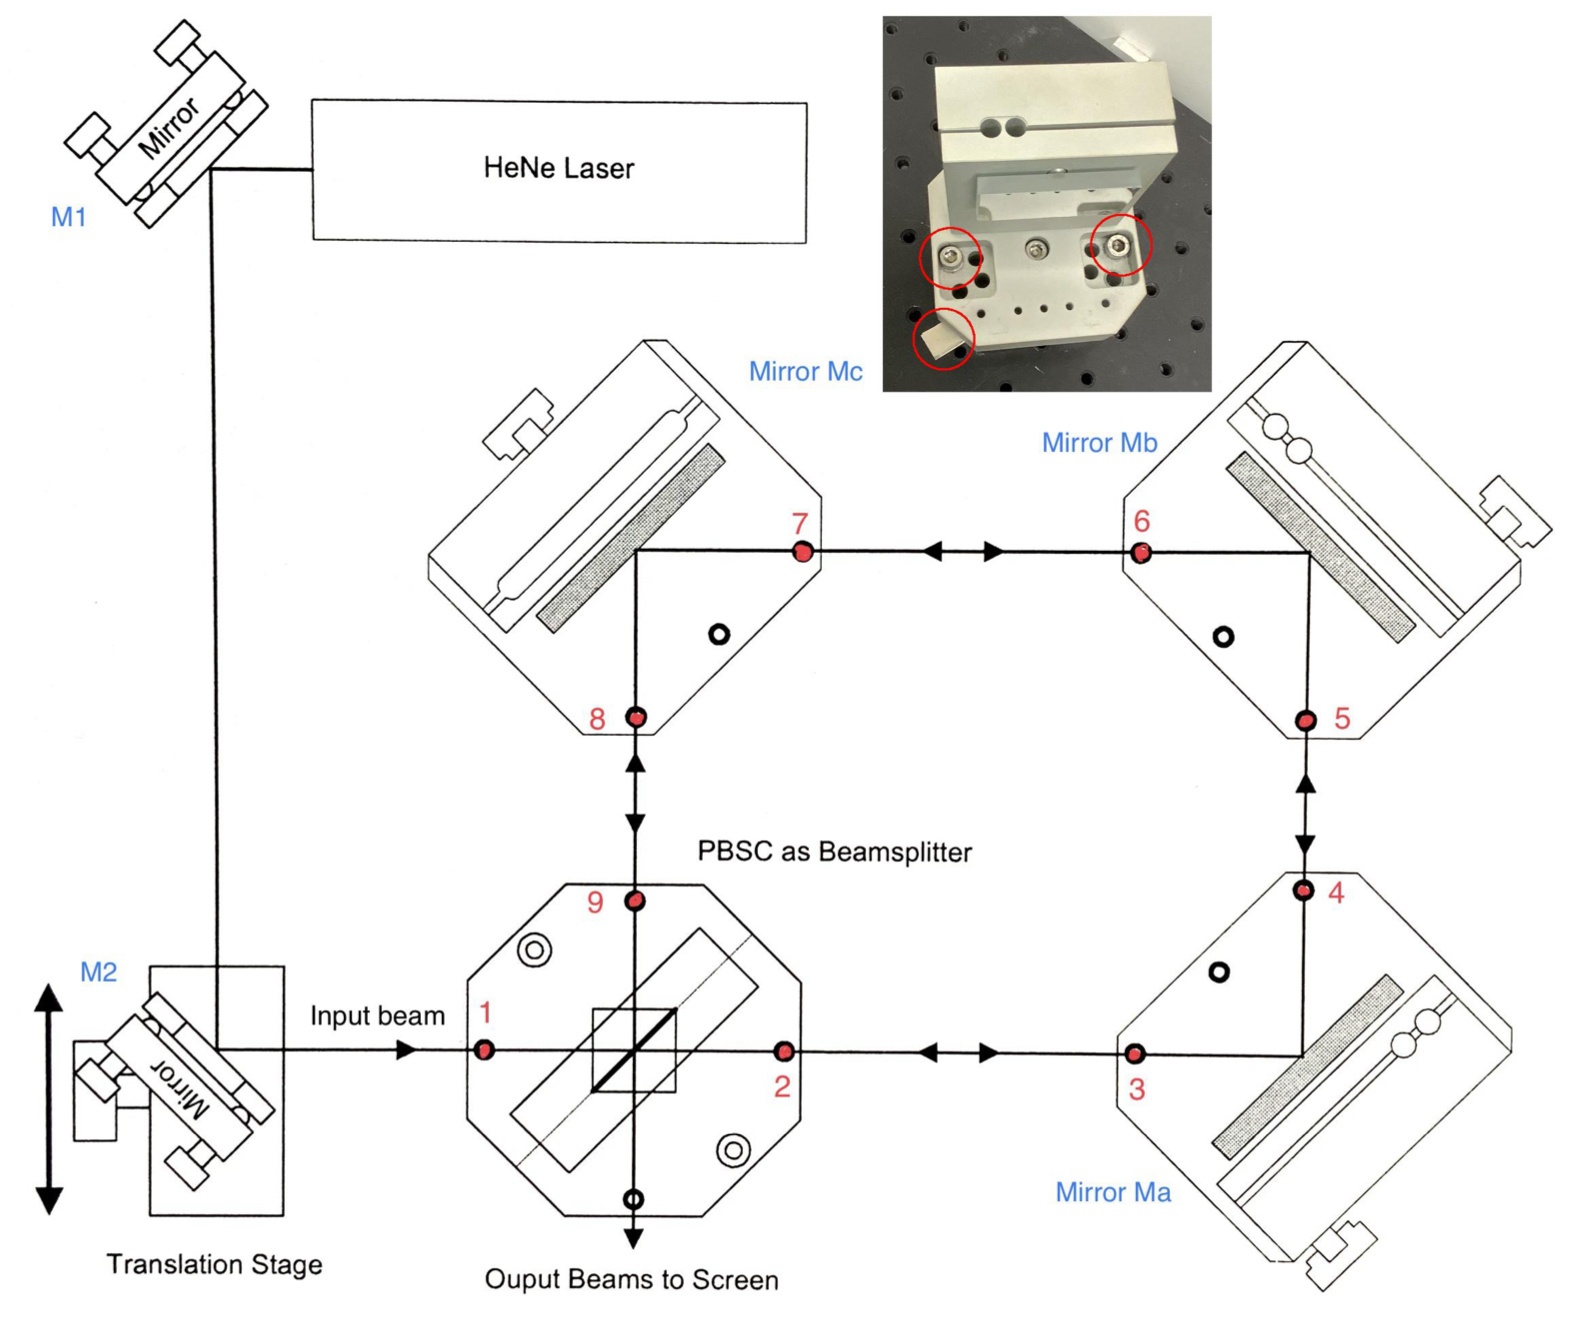
\includegraphics[width=0.70\textwidth]{content/Bilder/Sagnac_Interferometer.jpeg}
    \caption{Topology of the Sagnac-Interferometer}
    \label{pic:Sagnac-Interferometer}
  \end{figure}
